\newpage
\section{Graphics}

\subsection{First cluster}
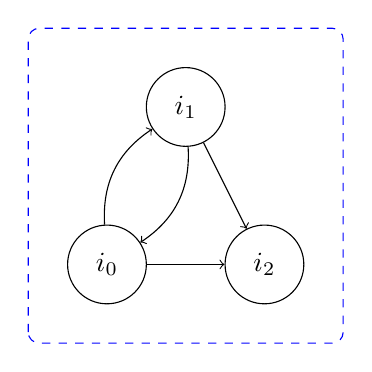
\begin{tikzpicture}[neuron/.style={circle, minimum size=1cm, draw=black!100}]
	\draw[rounded corners, blue, dashed] (0, 0) rectangle (4, 4);

	\node[neuron] (top) at (2, 3) {$i_1$};
 	\node[neuron] (bottom-left) at (1, 1) {$i_0$};
 	\node[neuron] (bottom-right) at (3, 1) {$i_2$};
 	
 	\draw[->] (bottom-left) edge [bend left] (top);
 	\draw[->] (top) edge [bend left] (bottom-left);
 	\draw[->] (top) -- (bottom-right);
 	\draw[->] (bottom-left) -- (bottom-right);
\end{tikzpicture}

\subsection{Second cluster}
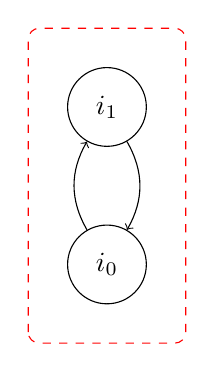
\begin{tikzpicture}[neuron/.style={circle, minimum size=1cm, draw=black!100}]
	\draw[rounded corners, red, dashed] (0, 0) rectangle (2, 4);
	
	\node[neuron] (top) at (1, 3) {$i_1$};
	\node[neuron] (bottom) at (1, 1) {$i_0$};
	
	\draw[->] (top) edge [bend left] (bottom);
	\draw[->] (bottom) edge [bend left] (top);
\end{tikzpicture}

\subsection{Second cluster placed on first cluster}
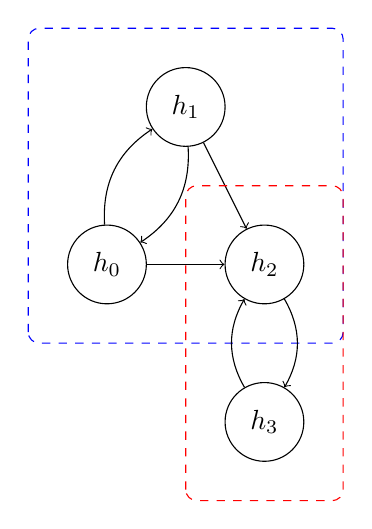
\begin{tikzpicture}[neuron/.style={circle, minimum size=1cm, draw=black!100}]
	\draw[rounded corners, blue, dashed] (0, 2) rectangle (4, 6);
	
	\node[neuron] (top) at (2, 5) {$h_1$};
	\node[neuron] (middle-left) at (1, 3) {$h_0$};
	\node[neuron] (middle-right) at (3, 3) {$h_2$};
	
	\draw[->] (middle-left) edge [bend left] (top);
	\draw[->] (top) edge [bend left] (middle-left);
	\draw[->] (top) -- (middle-right);
	\draw[->] (middle-left) -- (middle-right);

	\draw[rounded corners, red, dashed] (2, 0) rectangle (4, 4);

	\node[neuron] (bottom) at (3, 1) {$h_3$};
	
	\draw[->] (middle-right) edge [bend left] (bottom);
	\draw[->] (bottom) edge [bend left] (middle-right);
\end{tikzpicture}
